% Guia: Drones de resgate e a informação de Fisher
% Compile com XeLaTeX (recomendado) ou pdfLaTeX. No Overleaf: Menu > Compiler.
\documentclass[11pt,a4paper]{article}

\usepackage{iftex}
\ifXeTeX
  \usepackage{fontspec}
  \usepackage{polyglossia}
  \setdefaultlanguage[variant=brazilian]{portuguese}
  \setmainfont{Latin Modern Roman}
  \setsansfont{Latin Modern Sans}
  \setmonofont{Latin Modern Mono}
\else
  \usepackage[T1]{fontenc}
  \usepackage[utf8]{inputenc}
  \usepackage{lmodern}
  \usepackage[brazil]{babel}
\fi

\usepackage[a4paper,top=2.6cm,bottom=2.8cm,left=2.7cm,right=2.7cm,headheight=14pt]{geometry}
\usepackage{microtype}
\usepackage{amsmath,amssymb}
\usepackage{graphicx}
\usepackage{xcolor}
\usepackage{booktabs}
\usepackage{tabularx}
\usepackage{enumitem}
\usepackage{caption}
\usepackage{fancyhdr}
\usepackage{titlesec}
\usepackage[most]{tcolorbox}
\usepackage{csquotes}
\usepackage[hidelinks]{hyperref}

\graphicspath{{fig/}}

% ---------- cores ----------
\definecolor{azul}{HTML}{2A78D6}
\definecolor{azulclaro}{HTML}{EEF4FC}
\definecolor{laranja}{HTML}{D9480F}
\definecolor{cinza}{HTML}{56635B}
\definecolor{cinzaclaro}{HTML}{F3F5EF}
\definecolor{linha}{HTML}{C9D0C3}

% ---------- texto ----------
\setlength{\parindent}{0pt}
\setlength{\parskip}{0.55em}
\linespread{1.08}
\setlist{itemsep=0.25em,topsep=0.3em}
\captionsetup{font=small,labelfont=bf,labelsep=period,margin=0.5cm}
\renewcommand{\arraystretch}{1.25}

% ---------- títulos ----------
\titleformat{\section}{\Large\bfseries}{\thesection}{0.8em}{}
\titlespacing*{\section}{0pt}{2.2em}{0.8em}
\titleformat{\subsection}{\large\bfseries}{}{0em}{}
\titlespacing*{\subsection}{0pt}{1.4em}{0.4em}

% ---------- cabeçalho ----------
\pagestyle{fancy}
\fancyhf{}
\fancyhead[L]{\small\color{cinza}Drones de resgate e a informação de Fisher}
\fancyhead[R]{\small\color{cinza}\thepage}
\renewcommand{\headrulewidth}{0.3pt}

% ---------- quadros ----------
\newtcolorbox{noapp}{enhanced,colback=azulclaro,colframe=azulclaro,
  borderline west={2pt}{0pt}{azul},arc=0pt,left=10pt,right=10pt,top=6pt,bottom=6pt,
  fontupper=\small,before skip=0.9em,after skip=0.9em,
  title={No app},coltitle=azul,fonttitle=\small\bfseries,attach title to upper={\par\smallskip}}
\newtcolorbox{conta}{enhanced,colback=white,colframe=linha,boxrule=0.5pt,arc=2pt,
  left=10pt,right=10pt,top=6pt,bottom=6pt,fontupper=\small,before skip=0.9em,after skip=0.9em,
  title={Para quem quiser a conta},coltitle=cinza,fonttitle=\small\bfseries,attach title to upper={\par\smallskip}}
\newtcolorbox{ideia}{enhanced,colback=cinzaclaro,colframe=cinzaclaro,arc=2pt,
  left=10pt,right=10pt,top=7pt,bottom=7pt,before skip=0.9em,after skip=0.9em}

\begin{document}

% ================= capa =================
\begin{titlepage}
\vspace*{2.5cm}
{\Huge\bfseries Drones de resgate e a\\[0.3em] informação de Fisher\par}
\vspace{1.2em}
{\Large\color{cinza} Um guia sem jargão para entender a teoria por trás do projeto\par}
\vspace{2.5em}
\begin{minipage}{0.92\linewidth}
\large Este guia explica, em linguagem comum, o que é a matriz de Fisher, por que ela ajuda a decidir onde os drones devem voar e como o computador encontra a melhor posição. Não é preciso saber estatística para acompanhar.
\end{minipage}
\vfill
\begin{center}
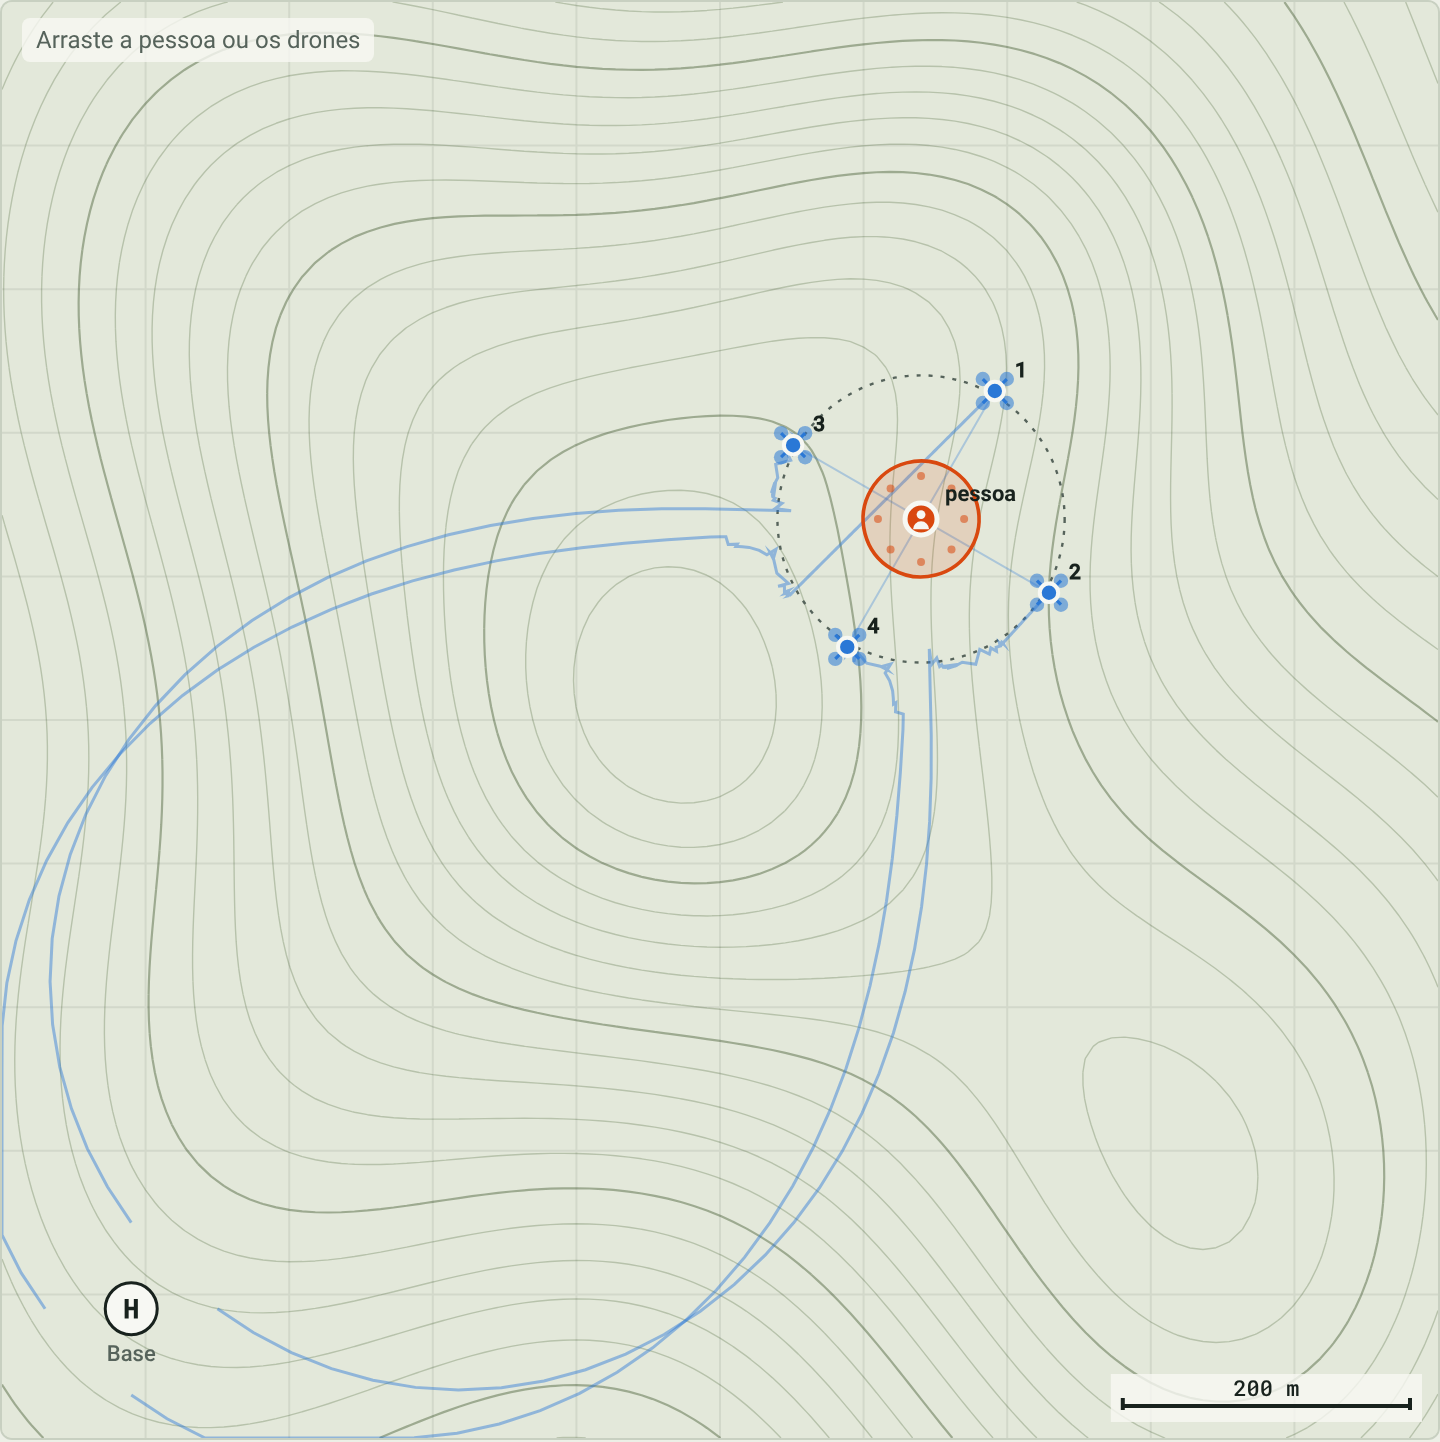
\includegraphics[width=0.52\linewidth]{app_posicionamento.png}\\[0.6em]
{\small\color{cinza} Quatro drones em volta da pessoa perdida, na posição que o app calculou como a melhor.}
\end{center}
\vspace{1cm}
\end{titlepage}

\setcounter{tocdepth}{1}
\tableofcontents
\thispagestyle{empty}
\clearpage

% ================= 1 =================
\section{A história do projeto}

Uma pessoa se perdeu numa área de mata de 1 km por 1 km. Ela não consegue dizer onde está, mas o celular dela continua ligado e emitindo sinal. Uma equipe de resgate lança alguns drones de uma base. Cada drone tem um receptor que mede a força do sinal do celular.

A força do sinal dá uma pista: quanto mais forte, mais perto o drone está da pessoa. Mas a pista é imprecisa. O sinal oscila por causa de árvores, relevo e da própria eletrônica, e duas medições no mesmo lugar dão valores diferentes.

A pergunta central do projeto é: \textbf{onde cada drone deve voar para descobrir a posição da pessoa com a maior precisão possível?}

Parece óbvio responder \enquote{voem até a pessoa}, mas não é. Um dos resultados mais interessantes do trabalho é que ficar bem em cima da pessoa é uma péssima posição para medir. Ao longo do guia vamos ver por quê.

\subsection{As três ideias do guia}
\begin{enumerate}
  \item \textbf{Medir é obter informação.} Algumas posições de medição informam muito mais do que outras. A \emph{informação de Fisher} é a régua que mede isso.
  \item \textbf{Escolher onde medir é um problema de otimização.} Queremos as posições que dão a maior informação total, respeitando limites como o alcance da bateria.
  \item \textbf{Depois de medir, estimamos a posição.} Procuramos o ponto do mapa que melhor explica as medições. Com essa estimativa, decidimos para onde voar em seguida, e o ciclo se repete.
\end{enumerate}

\begin{noapp}
O site do projeto tem quatro abas. \textbf{Posicionamento ótimo} mostra a ideia 2 com a posição da pessoa conhecida. \textbf{Missão de busca} junta tudo com a posição desconhecida. \textbf{Comparação} testa estratégias em dezenas de missões simuladas. \textbf{Teoria} tem a versão matemática completa. Este guia é a versão em linguagem comum.
\end{noapp}

Os capítulos vão do mais concreto ao mais abstrato. Quadros azuis como o de cima mostram onde ver cada ideia no app. Quadros com borda trazem a conta para quem quiser; dá para pular todos sem perder o fio.

% ================= 2 =================
\section{Medir com ruído}

Imagine que alguém está gritando numa praça cheia de gente e você tenta adivinhar a distância pela altura da voz. Perto, alguns passos fazem a voz mudar bastante. Longe, você pode andar um bocado e a voz parece igual. E o barulho da praça atrapalha sempre.

O sinal de celular funciona do mesmo jeito. A Figura~\ref{fig:sinal} mostra a força média do sinal que um drone, voando a 100 m de altura, recebe conforme se afasta da pessoa na horizontal. A faixa clara é o ruído: na prática, cada medição cai em algum lugar dessa faixa.

\begin{figure}[htbp]
  \centering
  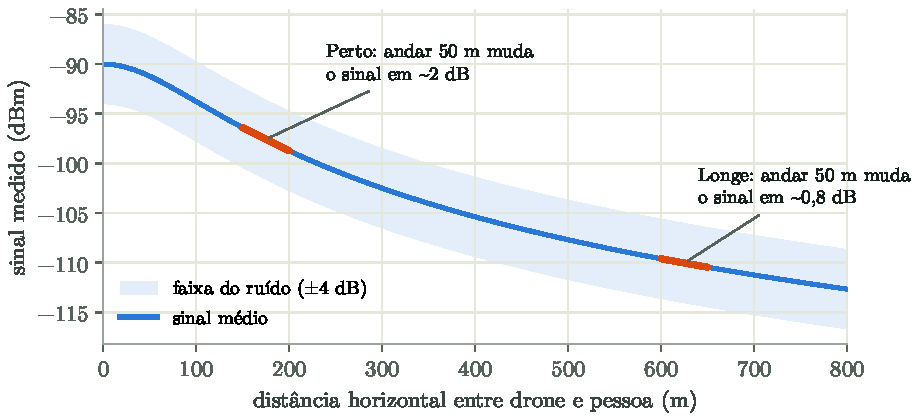
\includegraphics[width=0.9\linewidth]{sinal.pdf}
  \caption{Força do sinal contra a distância horizontal. O dBm é uma escala logarítmica de potência. Os trechos laranja mostram quanto o sinal muda quando a pessoa está 50 m mais longe: cerca de 2 dB perto do drone e menos de 1 dB longe dele. O ruído típico, de 4 dB para cima ou para baixo, engole facilmente essa mudança pequena.}
  \label{fig:sinal}
\end{figure}

Daqui sai a ideia mais importante do guia:

\begin{ideia}
\textbf{Uma medição é útil quando um pequeno deslocamento da pessoa muda bastante o valor medido, comparado com o tamanho do ruído.} Se a pessoa pode andar 50 m e o sinal mal se altera, a medição quase não ajuda a dizer onde ela está.
\end{ideia}

Existem duas forças em jogo. Uma é a inclinação da curva: quanto mais íngreme, melhor. A outra é o ruído: quanto menor, melhor. A informação de Fisher, na Seção~\ref{sec:fisher}, é exatamente a combinação dessas duas coisas.

\begin{conta}
O modelo usado é o de perda de percurso log-distância, comum em engenharia de rádio:
\[
  y = P_0 - 10\,\eta\,\log_{10} d + \varepsilon ,
\]
em que $y$ é o sinal medido, $d$ é a distância em linha reta entre drone e pessoa (contando a altura do voo), $P_0 = -40$~dBm é o sinal a 1 m, $\eta = 2{,}5$ diz quão rápido o sinal enfraquece e $\varepsilon$ é o ruído, com desvio-padrão de 4~dB.
\end{conta}

% ================= 3 =================
\section{Uma medição só diz \enquote{quão longe}}

O sinal não tem direção. Um drone sabe, aproximadamente, a que distância a pessoa está, mas não sabe se ela está ao norte, ao sul ou a leste. Todas as posições na mesma distância dão o mesmo sinal.

Por isso, uma medição sozinha só diz que a pessoa está em algum lugar de um anel ao redor do drone. O anel tem uma certa largura por causa do ruído.

\begin{figure}[htbp]
  \centering
  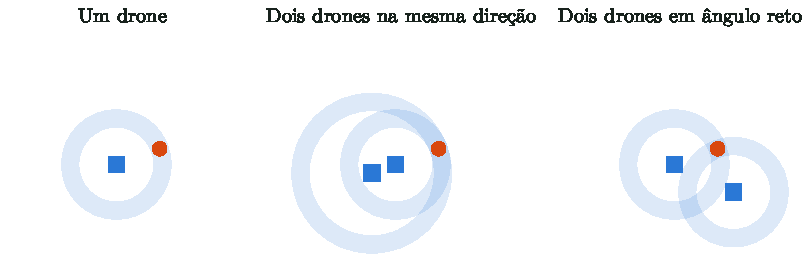
\includegraphics[width=0.95\linewidth]{aneis.pdf}
  \caption{O quadrado azul é o drone, o ponto laranja é a pessoa e o anel claro mostra onde ela pode estar segundo cada drone. Com dois drones na mesma direção, os anéis se sobrepõem numa faixa comprida. Com dois drones em ângulo reto, os anéis se cruzam num pedaço pequeno e a posição fica bem determinada.}
  \label{fig:aneis}
\end{figure}

Esse é o mesmo princípio da triangulação usada pelo GPS e pelas antenas de celular: \textbf{cada medidor fornece informação só numa direção, a da linha que o liga à pessoa.} Para localizar alguém num plano, é preciso olhar de direções diferentes.

Daqui já sai uma conclusão prática: mandar todos os drones juntos, em fila, é um desperdício. Eles medem praticamente a mesma coisa.

\begin{noapp}
Na aba Posicionamento ótimo, ligue \enquote{Mostrar onde um drone extra mais ajudaria}. O mapa pinta de azul os lugares onde um drone a mais acrescentaria mais informação. As regiões mais fortes ficam justamente nas direções que os drones atuais ainda não cobrem.
\end{noapp}

% ================= 4 =================
\section{A informação de Fisher, sem fórmulas}\label{sec:fisher}

Ronald Fisher foi um estatístico inglês do começo do século 20. Ele propôs uma forma de medir quanto um dado observado ensina sobre algo que não conseguimos ver diretamente. Em palavras simples:

\begin{ideia}
\textbf{Informação de Fisher} = quão sensível a medição é a uma mudança no que queremos descobrir, dividido pelo tamanho do ruído.

Elevamos ao quadrado para que mudanças para cima ou para baixo contem igual. Muita sensibilidade e pouco ruído significam muita informação.
\end{ideia}

No nosso caso, \enquote{o que queremos descobrir} é a posição da pessoa. Então a pergunta é: se a pessoa estivesse um pouquinho mais para o lado, quanto o sinal medido mudaria?

\subsection{Uma propriedade muito útil: informação se soma}
Se as medições têm ruídos independentes, a informação total é a soma da informação de cada uma. Dez medições no mesmo ponto dão dez vezes a informação de uma. Quatro drones somam a informação dos quatro. É isso que permite tratar o problema como \enquote{escolher as posições que somam mais informação}.

\subsection{Por que ficar em cima da pessoa é ruim}
Agora dá para entender a surpresa da Seção~1. Os drones voam a 100 m de altura. Se um drone está bem em cima da pessoa e ela anda um pouco para o lado, a distância entre os dois quase não muda, porque o movimento é perpendicular à linha que liga drone e pessoa (Figura~\ref{fig:altitude}).

\begin{figure}[htbp]
  \centering
  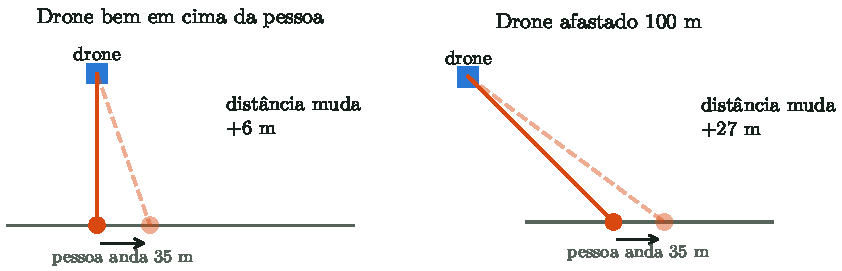
\includegraphics[width=0.88\linewidth]{altitude.pdf}
  \caption{Vista de lado. A pessoa anda 35 m. Com o drone bem em cima, a distância até ele aumenta só 6 m. Com o drone afastado 100 m na horizontal, aumenta 27 m. Mudança maior na distância significa mudança maior no sinal e, portanto, mais informação.}
  \label{fig:altitude}
\end{figure}

Do outro lado, longe demais, o sinal fica fraco e quase plano, como vimos na Seção~2. Existe então uma distância ideal no meio. A conta mostra que ela é exatamente igual à altitude de voo: com drones a 100 m de altura, a melhor distância horizontal é 100 m (Figura~\ref{fig:info}).

\begin{figure}[htbp]
  \centering
  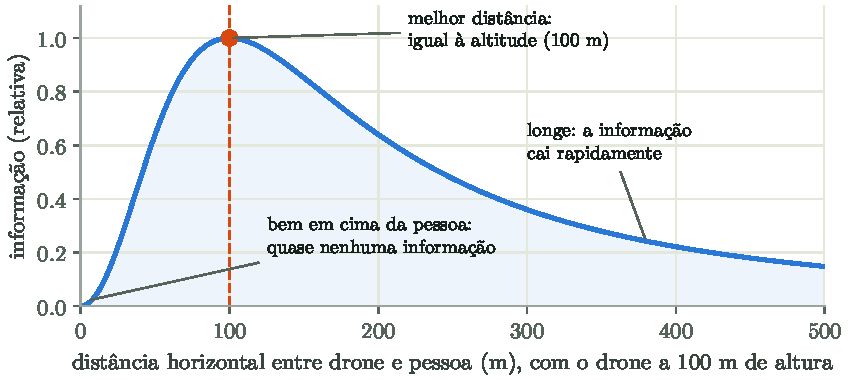
\includegraphics[width=0.9\linewidth]{info_r.pdf}
  \caption{Informação que um drone fornece conforme sua distância horizontal até a pessoa, com voo a 100 m de altura. O máximo fica em 100 m. Se a altitude mudar, o ponto ideal muda junto; dá para testar isso no app com o controle \enquote{Altitude de voo}.}
  \label{fig:info}
\end{figure}

\begin{conta}
Para um drone à distância horizontal $r$, voando à altura $h$, a informação é proporcional a
\[
  I(r) \propto \frac{r^2}{(r^2+h^2)^2}.
\]
Derivando em relação a $r^2$ e igualando a zero, $(r^2+h^2) - 2r^2 = 0$, ou seja, $r = h$.
\end{conta}

% ================= 5 =================
\section{De um número para uma matriz}

Até aqui falamos de \enquote{quanta informação}. Mas a posição da pessoa tem duas coordenadas, leste--oeste e norte--sul, e cada drone só informa na direção da linha que o liga à pessoa. Precisamos de algo que guarde quanto sabemos em cada direção.

A \textbf{matriz de Fisher} faz isso. É uma tabela $2\times 2$ de números que descreve quanta informação temos em qualquer direção do mapa. Não é preciso saber manipular matrizes para entender a ideia: pense nela como um resumo de \enquote{em que direções estamos bem informados e em quais estamos às cegas}.

\subsection{A elipse de incerteza}
Existe um jeito visual de enxergar a matriz. Invertendo-a, obtemos a \textbf{elipse de incerteza}: a região onde a pessoa provavelmente está, com 95\% de confiança.
\begin{itemize}
  \item Muita informação numa direção faz a elipse ficar estreita nessa direção.
  \item Pouca informação numa direção faz a elipse ficar comprida nessa direção.
  \item Informação parecida em todas as direções produz uma elipse redonda.
\end{itemize}

\begin{figure}[htbp]
  \centering
  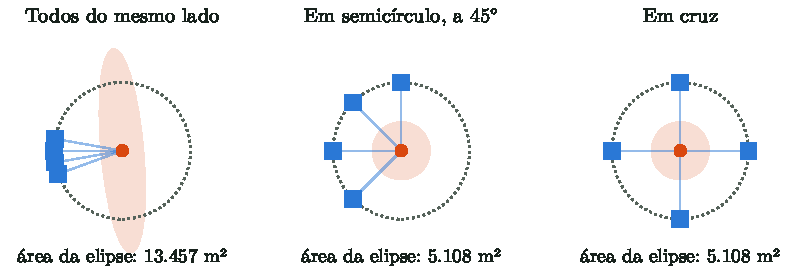
\includegraphics[width=0.95\linewidth]{elipses.pdf}
  \caption{Quatro drones a 100 m da pessoa, cada um com 10 medições, em três arranjos. Todos do mesmo lado: a elipse fica comprida, porque ninguém olha na direção perpendicular. Em semicírculo ou em cruz: a elipse fica redonda, com a mesma área de 5.108~m², menos da metade dos 13.457~m² do primeiro caso.}
  \label{fig:elipses}
\end{figure}

\subsection{O limite de Cramér--Rao: a melhor precisão possível}
Um resultado clássico da estatística, o limite de Cramér--Rao, diz o seguinte: \textbf{com essas medições, nenhum método de cálculo consegue ser mais preciso do que a elipse indica.} Ela é um piso para a incerteza. Métodos ruins ficam acima dela; bons métodos chegam perto.

Isso é poderoso porque permite avaliar uma posição de drones antes de voar. Não precisamos medir de verdade para saber quão boa ela seria: basta calcular a matriz de Fisher e olhar a elipse.

\subsection{Transformando a elipse em um número: o determinante}
Para comparar arranjos precisamos de um único número. O mais usado é o \textbf{determinante} da matriz de Fisher, e a interpretação é simples: quanto maior o determinante, menor a área da elipse. Maximizar o determinante é encolher a elipse. Esse critério se chama \textbf{D-ótimo}, com D de determinante, e é o que o projeto usa.

\begin{conta}
Com $v = p - q$ o vetor que vai do drone $q$ até a pessoa $p$, a matriz de Fisher de uma medição é
\[
  F_i = k\,\frac{v\,v^{\top}}{\left(\lVert v\rVert^2 + h^2\right)^2},
  \qquad k = \left(\frac{10\,\eta}{\sigma \ln 10}\right)^2 ,
\]
e a matriz total é a soma $F = \sum_i n_i F_i$, em que $n_i$ é o número de medições do drone $i$. A área da elipse é proporcional a $1/\sqrt{\det F}$. Na prática maximizamos $\log\det F$, que tem o mesmo ponto ótimo e é mais fácil de calcular.
\end{conta}

% ================= 6 =================
\section{O problema de otimização}

Agora temos tudo para escrever o problema do jeito que a disciplina ensina: variáveis de decisão, função objetivo e restrições.

\begin{table}[htbp]
\centering
\small
\begin{tabularx}{\linewidth}{@{}lX@{}}
\toprule
Ingrediente & No projeto \\
\midrule
Variáveis de decisão & A posição de cada drone no mapa, duas coordenadas por drone. Com 4 drones, são 8 números a escolher. \\
Função objetivo & Maximizar $\log\det F$, ou seja, deixar a elipse de incerteza a menor possível. \\
Restrição: área & Os drones não saem do mapa de 1 km $\times$ 1 km. \\
Restrição: bateria & Opcional. Cada drone fica a no máximo uma certa distância da base. \\
Restrição: segurança & Os drones não podem ficar a menos de 40 m um do outro. \\
\bottomrule
\end{tabularx}
\caption{Os ingredientes do problema de otimização.}
\end{table}

O problema é \textbf{não linear}, porque a informação depende das posições por meio de distâncias, quadrados e um determinante. Também é \textbf{não convexo}: o \enquote{terreno} da função objetivo tem vários morros, e nem todo topo é o mais alto. Isso vai importar na Seção~\ref{sec:armadilhas}.

\begin{conta}
Em notação de otimização, com $b$ a posição da base e $R$ o alcance da bateria:
\[
  \max_{q_1,\dots,q_N}\ \log\det F(q)
  \quad\text{sujeito a}\quad
  q_i \in [0,\,1000]^2,\quad
  \lVert q_i - b\rVert \le R,\quad
  \lVert q_i - q_j\rVert \ge 40 .
\]
\end{conta}

\subsection{Ligação com a disciplina}
\begin{table}[htbp]
\centering
\small
\begin{tabularx}{\linewidth}{@{}p{0.36\linewidth}X@{}}
\toprule
Assunto da disciplina & Onde aparece no projeto \\
\midrule
Programação não linear & O problema inteiro: objetivo não linear com restrições. \\
Método do gradiente & Os drones \enquote{sobem o morro} da informação seguindo o gradiente. \\
Descida com otimização do comprimento do passo & A busca de Armijo decide o tamanho de cada passo. \\
Lagrange e condições de otimalidade & Multiplicadores que medem quanto a restrição da bateria \enquote{empurra} cada drone. \\
Métodos de segunda ordem & Gauss--Newton, ou Fisher scoring, para estimar a posição da pessoa. \\
Métodos numéricos & Busca em grade e múltiplos pontos de partida para escapar de ótimos locais. \\
\bottomrule
\end{tabularx}
\caption{Onde cada assunto da disciplina aparece no projeto.}
\end{table}

% ================= 7 =================
\section{Como o computador acha o melhor lugar}

Imagine que você está num morro coberto de neblina e quer chegar ao topo. Você não enxerga o topo, mas sente com os pés para que lado o chão sobe mais. Você dá um passo nessa direção, sente de novo, dá outro passo. Isso é o método do gradiente.

O \textbf{gradiente} é justamente essa informação: para cada drone, ele diz em que direção mover o drone aumenta mais a informação total, e quão rápido ela aumenta. O computador calcula o gradiente, move todos os drones um pouco nessa direção e repete até que nenhum movimento pequeno melhore mais nada.

\begin{figure}[htbp]
  \centering
  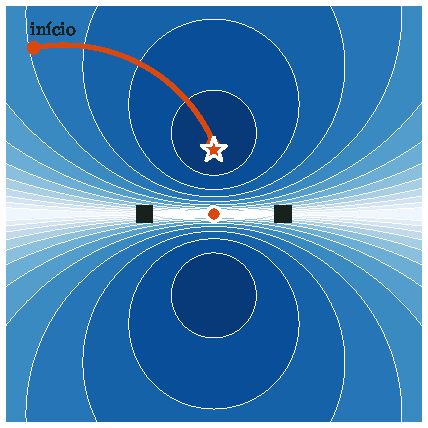
\includegraphics[width=0.55\linewidth]{paisagem.pdf}
  \caption{Dois drones (quadrados pretos) já estão à esquerda e à direita da pessoa (ponto laranja). As cores mostram quanta informação um terceiro drone acrescentaria em cada ponto: mais escuro é melhor. As melhores regiões ficam acima e abaixo da pessoa, nas direções ainda não cobertas. A linha laranja é o caminho que o método do gradiente faz a partir do canto, até a estrela.}
  \label{fig:paisagem}
\end{figure}

\subsection{O tamanho do passo}
Saber a direção não basta. Passos grandes demais podem pular o topo e cair do outro lado, mais baixo. Passos pequenos demais fazem a subida durar uma eternidade (Figura~\ref{fig:passo}).

\begin{figure}[htbp]
  \centering
  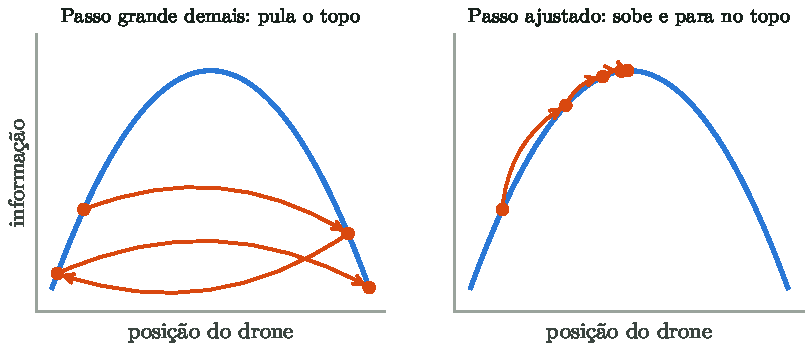
\includegraphics[width=0.9\linewidth]{passo.pdf}
  \caption{À esquerda, com passo fixo e grande, o drone pula de um lado para o outro do topo sem chegar. À direita, com o passo ajustado, ele sobe e para no topo.}
  \label{fig:passo}
\end{figure}

O app usa a \textbf{regra de Armijo}: tenta um passo; se a informação aumentou o suficiente, aceita e no próximo tenta um passo maior; se não aumentou, corta o passo pela metade e tenta de novo. Além disso, nenhum drone anda mais de 30 m por iteração, como se fosse uma velocidade máxima.

\subsection{Restrições: a cerca e as molas}
\begin{itemize}
  \item \textbf{Área e bateria} funcionam como uma cerca. Se o passo levaria um drone para fora, ele é trazido de volta para o ponto mais próximo dentro da cerca. Isso se chama \emph{projeção}.
  \item \textbf{Distância mínima entre drones} funciona como uma mola. Se dois drones chegam perto demais, a função objetivo recebe uma penalidade que cresce com a invasão e empurra os dois para longe.
\end{itemize}

Quando um drone termina encostado na cerca da bateria, as \textbf{condições de KKT}, a versão das condições de Lagrange para restrições do tipo \enquote{no máximo}, dizem como reconhecer que ele está no lugar certo. O gradiente dele precisa apontar para fora da cerca: ele queria ir mais longe, mas não pode. E não pode haver nenhuma vontade de deslizar ao longo da cerca.

O \textbf{multiplicador $\lambda$} mede a força com que o drone empurra a cerca. Se $\lambda$ é grande, aumentar o alcance da bateria traria muito ganho.

\begin{conta}
Para um drone parado na fronteira $\lVert q_i - b\rVert = R$, a condição de KKT é
\[
  \nabla_{q_i} \log\det F = \lambda_i\,\frac{q_i - b}{\lVert q_i - b\rVert},
  \qquad \lambda_i \ge 0 .
\]
Para um drone livre, no meio do mapa, a condição é simplesmente $\nabla_{q_i}\log\det F = 0$.
\end{conta}

\begin{noapp}
Escolha o cenário \enquote{Bateria limitada}. Os drones param no círculo tracejado e a tabela \enquote{Condições de KKT} mostra $\lambda$ positivo e gradiente ao longo da cerca praticamente zero para cada um. Troque o otimizador para \enquote{passo fixo} e aumente o passo: você verá o zigue-zague do lado esquerdo da Figura~\ref{fig:passo}.
\end{noapp}

% ================= 8 =================
\section{Armadilhas e como o app escapa delas}\label{sec:armadilhas}

Construir o app revelou três problemas que não aparecem nos exemplos de livro. Todos têm a ver com o fato de o problema ser não convexo e com as limitações do método do gradiente. São bons assuntos para a apresentação, porque mostram a teoria funcionando, e às vezes falhando, na prática.

\subsection{Armadilha 1: empates e posições frágeis}
Na Figura~\ref{fig:elipses}, o semicírculo e a cruz têm exatamente a mesma elipse. Para a matemática, são igualmente bons. Mas o semicírculo é frágil: se a pessoa estiver uns 30 a 60 m fora do lugar que supusemos, ele perde mais informação do que a cruz.

\textbf{Solução: o critério robusto.} Em vez de calcular a informação só no ponto exato onde achamos que a pessoa está, o app calcula a média sobre vários pontos próximos, num raio de 30 m. Na prática: não apostar tudo num único palpite. Isso desfaz o empate e a cruz passa a ganhar. O nome técnico é \emph{projeto bayesiano de experimentos}.

\subsection{Armadilha 2: ótimos locais}
Os drones saem todos da base, então chegam pelo mesmo lado. O método do gradiente só olha para o chão logo abaixo dos pés: ele fica satisfeito com o primeiro topo que encontra, mesmo que exista um mais alto do outro lado do vale. No nosso caso, isso deixava os drones amontoados do lado da base.

\textbf{Solução: multistart.} Quando o gradiente para, o app recomeça a subida a partir de 16 arranjos iniciais diferentes e fica com o melhor resultado. Se ele for melhor que o atual, os drones voam até lá. É a forma mais simples, e muito usada, de lidar com problemas que têm vários morros.

\subsection{Armadilha 3: drones distantes ficam para trás}
No método do gradiente puro, todos os drones andam com o mesmo passo, e o tamanho desse passo é limitado pelo drone que tem o gradiente maior. Um drone distante tem gradiente muito menor, porque longe da pessoa tudo muda devagar. Com isso, ele se arrasta: nos testes, dois drones chegavam perto da pessoa só por volta da iteração 130, enquanto os outros chegavam na 27.

A função objetivo estava certa. O gradiente foi conferido contra uma aproximação numérica e bate até a 9ª casa decimal. O problema era de escala, uma fraqueza clássica do método do gradiente.

\textbf{Solução: passo por drone.} O app passou a ajustar a escala do passo de cada drone separadamente, sempre com o limite de 30 m por iteração. Agora todos chegam por volta da iteração 28. O nome técnico é \emph{pré-condicionamento}.

\begin{figure}[htbp]
  \centering
  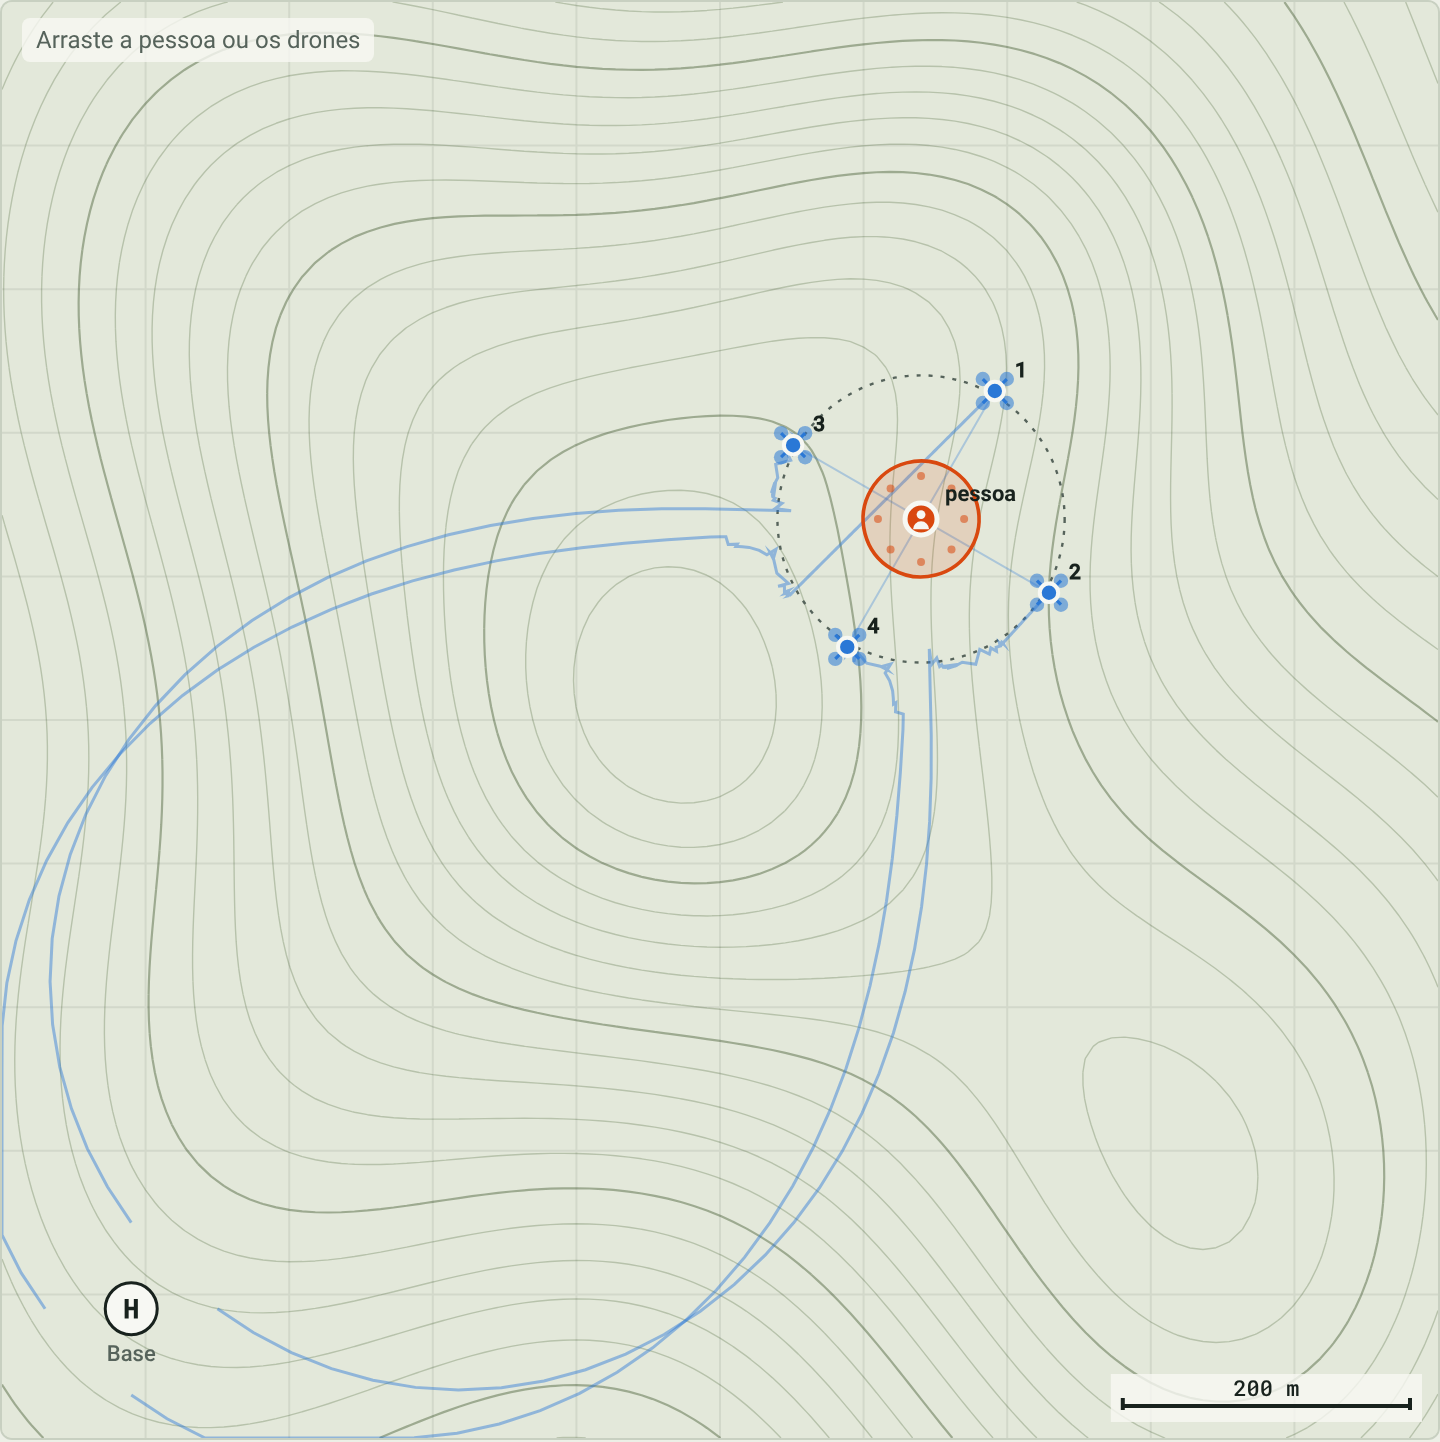
\includegraphics[width=0.58\linewidth]{app_posicionamento.png}
  \caption{Resultado final no app, com as três soluções ativas: quatro drones em cruz, a cerca de 103 m da pessoa (um pouco mais que os 100 m teóricos, efeito do critério robusto). As linhas azuis são os caminhos percorridos desde a base. Os pontinhos laranja em volta da pessoa são a nuvem de posições usada pelo critério robusto.}
\end{figure}

% ================= 9 =================
\section{A missão: achar quem não sabemos onde está}

Até aqui supusemos que sabíamos onde a pessoa está, para entender quais posições de drone são boas. Na vida real é o contrário: não sabemos, e é isso que queremos descobrir. A aba Missão de busca resolve esse problema com um ciclo de quatro passos.

\begin{enumerate}
  \item \textbf{Medir.} Cada drone faz 5 medições do sinal onde está.
  \item \textbf{Estimar.} Com todas as medições feitas até agora, o computador calcula o ponto mais provável para a pessoa.
  \item \textbf{Planejar.} Usando esse ponto estimado no lugar da posição verdadeira, ele escolhe para onde cada drone deve ir, maximizando a informação como nas seções anteriores. Cada drone só pode voar 150 m por rodada.
  \item \textbf{Voar.} Os drones vão para as novas posições e o ciclo recomeça.
\end{enumerate}

\subsection{Estimar: qual posição explica melhor as medições?}
A ideia se chama \textbf{máxima verossimilhança}. Para cada ponto do mapa, o computador pergunta: se a pessoa estivesse aqui, quão parecidas com o que medimos seriam as medições esperadas? O ponto onde as medições ficam menos surpreendentes é a estimativa.

No app, isso aparece como uma mancha laranja no mapa: quanto mais forte, mais compatível o ponto é com as medições. Nas primeiras rodadas a mancha é um arco comprido, porque os drones ainda estão juntos e só sabem a distância. Conforme eles se espalham, a mancha encolhe até virar uma pequena região.

\subsection{Um atalho de segunda ordem}
Para achar o melhor ponto com precisão, o app primeiro testa uma grade de $60 \times 60$ pontos e depois refina. O refinamento poderia ser feito pelo método do gradiente, mas há um caminho mais esperto: o \textbf{método de Gauss--Newton}. Ele usa, além da inclinação, a curvatura do terreno. É como saber não só para que lado o chão desce, mas também o formato do vale, o que permite pular quase direto para o fundo.

No nosso problema, Gauss--Newton coincide com o \textbf{Fisher scoring}, que usa a própria matriz de Fisher como medida de curvatura. Nos testes, ele chega a menos de 1 cm do ponto ótimo em 2 a 5 iterações, enquanto o gradiente precisa de dezenas.

\begin{conta}
A estimativa minimiza a soma dos quadrados dos resíduos, $S(p) = \sum_j \bigl(y_j - \mu_j(p)\bigr)^2$, em que $\mu_j(p)$ é o sinal esperado se a pessoa estivesse em $p$. Cada passo de Fisher scoring é
\[
  p^{k+1} = p^k + F(p^k)^{-1}\,\nabla \ell(p^k),
\]
em que $\ell$ é o logaritmo da verossimilhança. Com ruído gaussiano, isso é exatamente o passo de Gauss--Newton.
\end{conta}

\begin{figure}[htbp]
  \centering
  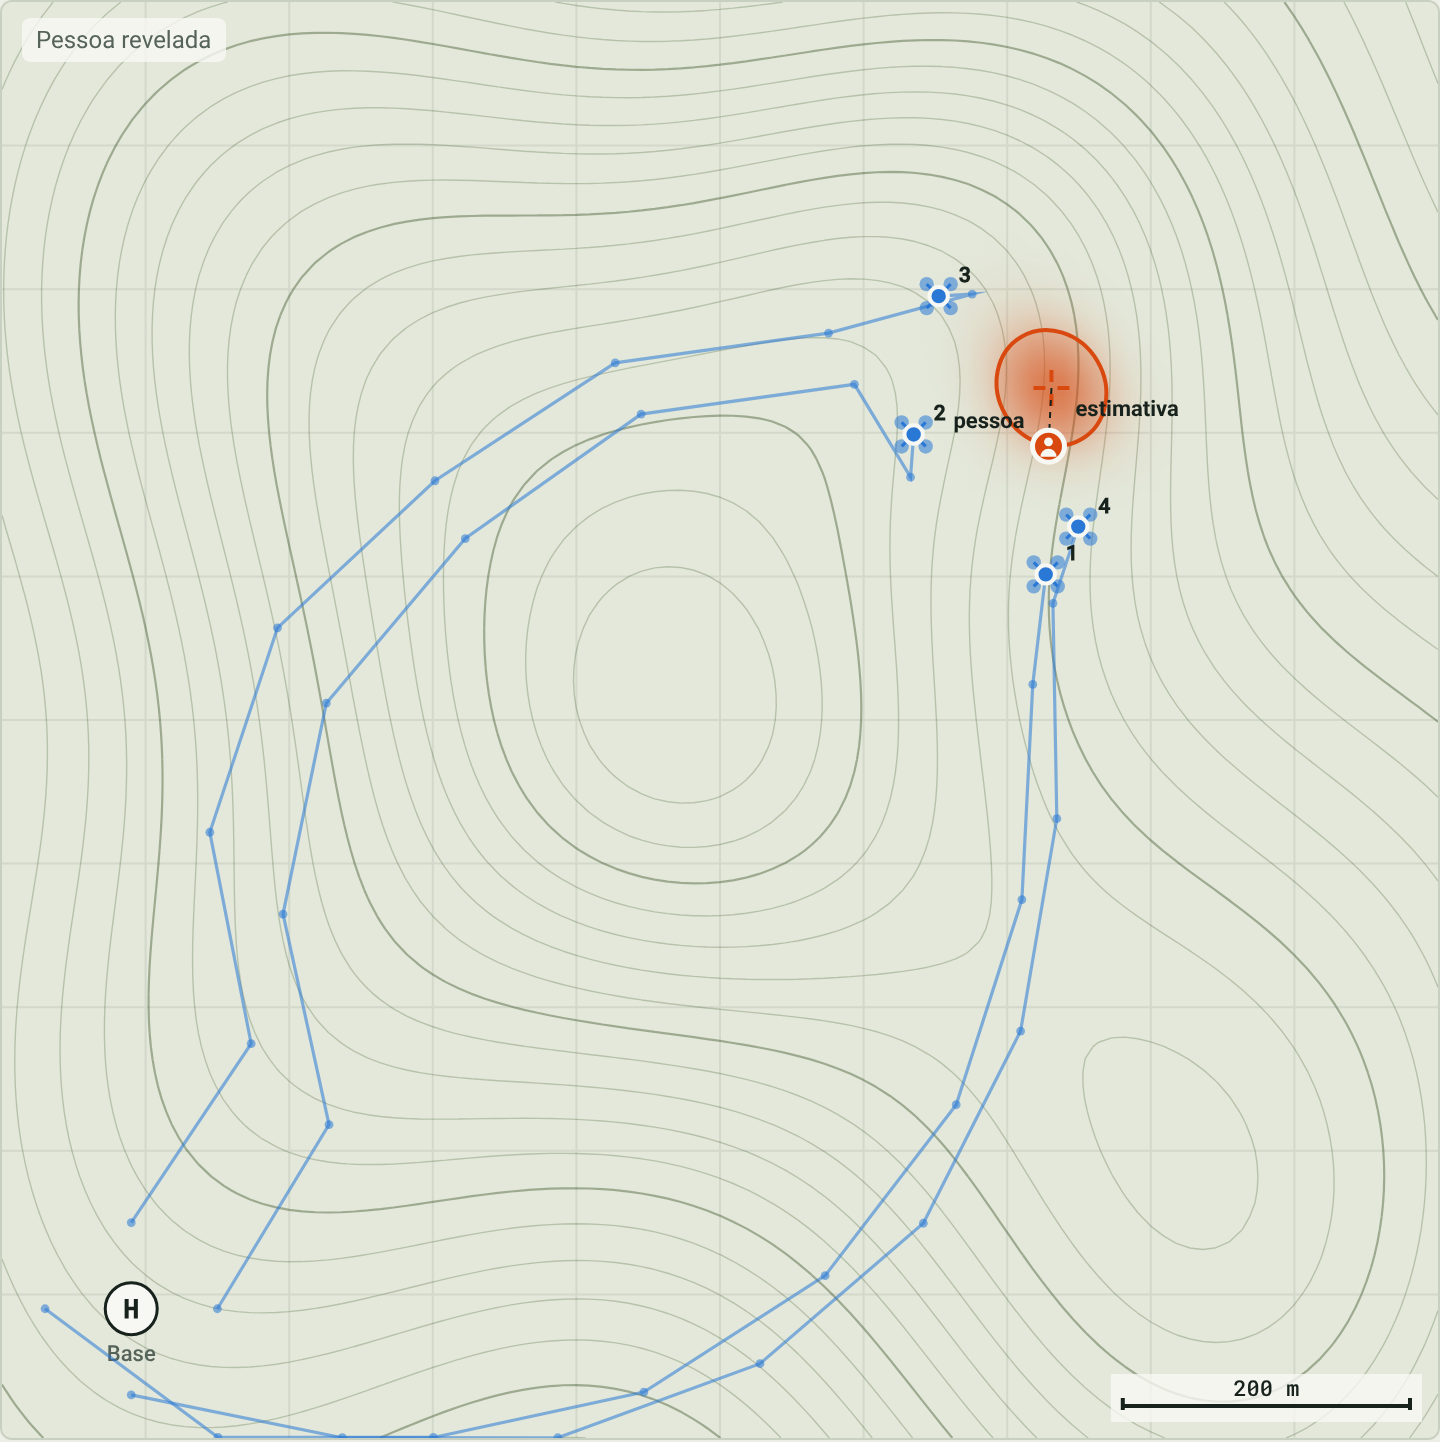
\includegraphics[width=0.58\linewidth]{app_missao.png}
  \caption{Uma missão na rodada 8, com a pessoa revelada. As linhas azuis são os trajetos desde a base, a cruz laranja é a estimativa e o círculo laranja é a elipse de 95\%. Nesta missão, a estimativa errou por 41 m e a pessoa ficou fora da elipse.}
  \label{fig:missao}
\end{figure}

\begin{ideia}
A Figura~\ref{fig:missao} mostra algo importante: \textbf{a elipse pode ser otimista.} O limite de Cramér--Rao vale de forma exata quando há muitas medições. Com poucas, ou quando a estimativa ainda está longe da verdade, o erro real pode passar da elipse. O app mostra os dois números lado a lado, \enquote{Incerteza} e \enquote{Erro real}, justamente para dar para comparar.
\end{ideia}

% ================= 10 =================
\section{O que os testes mostraram}

Uma missão sozinha depende da sorte: onde a pessoa estava e como o ruído caiu. Para comparar de forma justa, a aba Comparação roda 40 missões por grupo, e todos os grupos enfrentam as mesmas 40 pessoas perdidas e o mesmo ruído. O gráfico mostra o \emph{erro mediano}: metade das missões erra menos do que isso.

\begin{figure}[htbp]
  \centering
  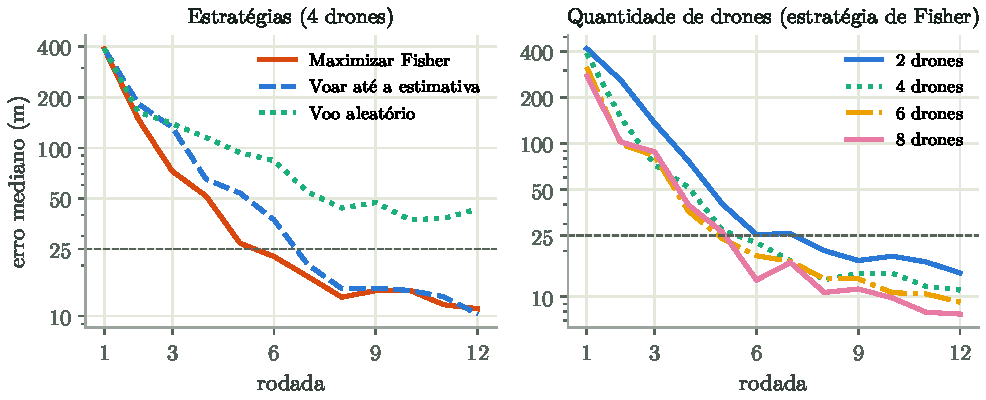
\includegraphics[width=\linewidth]{resultados.pdf}
  \caption{Erro mediano por rodada, em escala logarítmica. A linha tracejada marca 25 m. À esquerda, três estratégias com 4 drones. À direita, a estratégia de Fisher com 2, 4, 6 e 8 drones.}
  \label{fig:resultados}
\end{figure}

\subsection{Estratégias}
\begin{table}[htbp]
\centering
\small
\begin{tabular}{@{}lrrrr@{}}
\toprule
Estratégia (4 drones) & Rodada 3 & Rodada 6 & Rodada 12 & Abaixo de 25 m na rodada 6 \\
\midrule
Maximizar Fisher & 73 m & 23 m & 11 m & 55\% \\
Voar até a estimativa & 133 m & 37 m & 10 m & 45\% \\
Voo aleatório & 139 m & 84 m & 43 m & 20\% \\
\bottomrule
\end{tabular}
\caption{Erro mediano por estratégia, em 40 missões simuladas.}
\end{table}

A estratégia de Fisher chega mais rápido a uma boa precisão: na rodada 3, o erro dela é praticamente metade do das outras. No fim da missão, \enquote{voar até a estimativa} alcança o mesmo nível. A vantagem do método está na velocidade, o que num resgate pode ser decisivo.

A diferença é real, mas não é enorme em todas as métricas. Na fração de missões abaixo de 25 m na rodada 6, a vantagem é de 10 pontos percentuais. Com 40 missões há algum ruído estatístico nesses números.

\subsection{Quantidade de drones}
\begin{table}[htbp]
\centering
\small
\begin{tabular}{@{}lrrr@{}}
\toprule
Drones & Rodada 6 & Rodada 12 & Medições por rodada \\
\midrule
2 & 26 m & 14 m & 10 \\
4 & 23 m & 11 m & 20 \\
6 & 19 m & 9 m & 30 \\
8 & 13 m & 8 m & 40 \\
\bottomrule
\end{tabular}
\caption{Erro mediano com a estratégia de Fisher, por quantidade de drones.}
\end{table}

Mais drones ajudam, mas com \textbf{retorno decrescente}. Como a informação se soma, dobrar o número de drones dobra a informação. Só que o erro cai com a raiz quadrada da informação, e não na mesma proporção. Dobrar os drones reduz o erro em cerca de 30\%, não pela metade. Para cortar o erro pela metade, é preciso quadruplicar os drones.

A simulação confirma: na rodada 12, 8 drones têm cerca de 55\% do erro de 2 drones, e a teoria prevê 50\%. É o mesmo motivo pelo qual uma pesquisa eleitoral com 4 vezes mais entrevistados tem só metade da margem de erro.

% ================= 11 =================
\section{Onde o modelo simplifica}

Todo modelo simplifica a realidade. É importante saber onde, até para responder às perguntas do professor.

\begin{itemize}
  \item \textbf{O sinal real é mais bagunçado.} Celulares de verdade sofrem com relevo, vegetação, reflexões e a posição da antena. O ruído real costuma ser maior e menos previsível do que os 4 dB do modelo.
  \item \textbf{A informação depende da resposta que procuramos.} Para calcular a matriz de Fisher precisamos da posição da pessoa, que é justamente o que não sabemos. O app usa a estimativa atual, que pode estar errada nas primeiras rodadas. O critério robusto ameniza, mas não elimina, esse problema.
  \item \textbf{A elipse é uma promessa para muitas medições.} Com poucas medições, o erro real pode ser maior, como vimos na Figura~\ref{fig:missao}.
  \item \textbf{O planejamento olha só uma rodada à frente.} Ele escolhe a melhor próxima posição sem pensar nas rodadas seguintes. Planejar várias rodadas de uma vez seria melhor, porém muito mais caro de calcular.
  \item \textbf{O gradiente encontra ótimos locais.} O multistart aumenta a chance de achar o melhor, mas não garante.
  \item \textbf{A pessoa está parada} e o terreno não bloqueia voo nem sinal.
\end{itemize}

% ================= 12 =================
\section{Glossário}

\begin{description}[style=nextline,leftmargin=0pt,itemsep=0.45em,font=\normalfont\bfseries]
  \item[dBm] Unidade de potência de sinal em escala logarítmica. Quanto mais negativo, mais fraco. Cada 10 dB a menos significa 10 vezes menos potência.
  \item[Ruído] A variação aleatória que faz duas medições no mesmo lugar darem valores diferentes.
  \item[Informação de Fisher] Mede quanto uma medição ensina sobre algo desconhecido: a sensibilidade da medição a esse algo, ao quadrado, dividida pelo tamanho do ruído ao quadrado.
  \item[Matriz de Fisher] A versão da informação de Fisher para mais de uma incógnita. Aqui, uma tabela $2\times2$ que diz quanto sabemos em cada direção do mapa.
  \item[Elipse de incerteza (95\%)] A região onde a pessoa provavelmente está. Comprida na direção em que sabemos pouco, estreita onde sabemos muito.
  \item[Limite de Cramér--Rao] Teorema que garante que nenhum método consegue ser mais preciso do que o inverso da matriz de Fisher. É o piso da incerteza.
  \item[Determinante e critério D-ótimo] Um número que resume a matriz. Maximizar o determinante é o mesmo que minimizar a área da elipse.
  \item[Gradiente] A direção em que uma função cresce mais rápido, junto com a velocidade desse crescimento. É o \enquote{para que lado o morro sobe}.
  \item[Busca de Armijo] Regra para escolher o tamanho do passo: tenta, e se não melhorar o suficiente, corta pela metade.
  \item[Projeção] Trazer de volta para dentro da área permitida um ponto que saiu dela.
  \item[Condições de KKT e multiplicador $\lambda$] Regras que reconhecem um ótimo quando há restrições do tipo \enquote{no máximo}. O $\lambda$ mede o quanto a restrição está atrapalhando.
  \item[Ótimo local] Um ponto melhor que todos os vizinhos, mas não necessariamente o melhor de todos. Um topo de morro que não é o mais alto.
  \item[Multistart] Rodar a otimização a partir de vários pontos iniciais e ficar com o melhor resultado.
  \item[Pré-condicionamento] Reescalar as variáveis para que todas avancem num ritmo parecido durante a otimização.
  \item[Máxima verossimilhança] Escolher como estimativa o valor que torna os dados observados mais prováveis.
  \item[Gauss--Newton e Fisher scoring] Métodos de segunda ordem, que usam a curvatura além da inclinação e por isso convergem em poucas iterações. Neste problema, os dois são o mesmo método.
  \item[Projeto bayesiano (critério robusto)] Escolher onde medir levando em conta que não sabemos exatamente onde está o que procuramos, fazendo a média sobre as possibilidades.
  \item[Monte Carlo] Avaliar um método repetindo muitas simulações com sorteios diferentes e olhando as estatísticas dos resultados.
\end{description}

% ================= 13 =================
\section{Roteiro para a apresentação}

Uma sugestão de demonstração ao vivo, de 6 a 8 minutos, seguindo a ordem deste guia.

\begin{enumerate}[itemsep=0.5em]
  \item \textbf{O problema.} Abra a aba Missão de busca e mostre a situação: pessoa desconhecida, drones na base, sinal com ruído.
  \item \textbf{Uma medição só diz a distância.} Com a missão na rodada 1, mostre a mancha laranja em forma de arco. É o anel da Seção~3.
  \item \textbf{O que é informação.} Vá para Posicionamento ótimo. Arraste a pessoa e mostre os drones se reorganizando. Aponte o anel pontilhado: a distância ideal é igual à altitude. Mude a altitude e veja o anel e os drones acompanharem.
  \item \textbf{Elipse e Cramér--Rao.} Mostre o quadro \enquote{Elipse de incerteza}. Escolha \enquote{Dois drones} e depois \enquote{Seis drones} e compare o tamanho da elipse.
  \item \textbf{Otimização e restrições.} Escolha \enquote{Bateria limitada} e mostre a tabela de KKT com $\lambda$ positivo.
  \item \textbf{Armadilhas.} Troque \enquote{Limite de 30 m por iteração} para \enquote{Passo comum} e clique em \enquote{Voltar à base}: dois drones vão ficar para trás. Volte para \enquote{Por drone} e repita.
  \item \textbf{A missão completa.} Na aba Missão, clique em \enquote{Automático} e deixe rodar. No fim, marque \enquote{Revelar a pessoa}.
  \item \textbf{Os números.} Na aba Comparação, mostre o gráfico das estratégias e depois o de quantidade de drones. Feche com o retorno decrescente: o dobro de drones não divide o erro pela metade.
\end{enumerate}

\begin{ideia}
\textbf{Uma frase para fechar:} a matriz de Fisher permite medir quanto cada posição de drone vai ensinar antes de voar, e a otimização transforma isso numa decisão de onde voar.
\end{ideia}

\end{document}
